%Tim Dixon
%%Main takeaway - we provide calving front locations, and have automated it
%Some may be more interested in the data, or the method, so make sure we cover both

\documentclass[tc, manuscript]{copernicus}

\usepackage{wrapfig}

\begin{document}

\title{Calving Front Machine (CALFIN): Automated Calving Front Mask Dataset and Methodology for East/West Greenland, 1972-2019}

\Author[1]{Daniel}{Cheng}
\Author[1]{Yara}{Mohajerani}
\Author[2]{Michael}{Wood}
\Author[1]{Isabella}{Velicogna}
\Author[2]{Eric}{Larour}
\Author[1]{Wayne}{Hayes}

\affil[1]{University of California at Irvine, Irvine CA, USA}
\affil[2]{Jet Propulsion Laboratory, California Institute of Technology, Pasadena CA, USA}

\runningtitle{TEXT}

\runningauthor{TEXT}

\correspondence{Daniel Cheng (dlcheng@uci.edu)}

\received{}
\pubdiscuss{} %% only important for two-stage journals
\revised{}
\accepted{}
\published{}

\maketitle

\begin{abstract}
We present Calving Front Machine (CALFIN), a dataset of calving front masks for glaciers along West Greenland. The dataset is generated from Landsat imagery over the period 1972 to 2019. This dataset is unique in scope, and provides new constraints on glacial evolution over the time period. The current iteration offers a new opportunity to explore previous trends and validate existing models, enabling more accurate predictions moving forward.

The dataset is contains data that is automatically generated. We generate the vectorized calving fronts from raw Landsat imagery. Our method utilizes deep learning in the form of a neural network. This approach builds on existing work \citep{mohajerani2019} \citep{zhang2019} \citep{baumhoer2019}. The network itself is derived from U-Net/DeeplabV3+ Xception architectures \citep{ronneberger2015} \citep{chen2018} . Additional post-processing techniques allow our method to achieve accurate and useful segmentation of raw images into Shapefile outputs. This methodology is uniquely robust to clouds, illumination differences, ice mélange, and Landsat-7 scan-line errors/data coverage gaps.

We perform an analysis of CALFIN results, which approach human levels of accuracy in comparison to manually delineated fronts. Additionally, we perform a model inter-comparison to evaluate the robustness of CALFIN's performance and cross-validate it against existing methodologies. %TODO/Save for future paper? We show the applicability of CALFIN's methodology to SAR data, Antarctic glaciers, as well as non-marine terminating glaciers.

At this stage, we seek feedback from the community and welcome any critiques or questions regarding the dataset and/or our methods. This work was conducted as a collaboration between NASA’s Jet Propulsion Laboratory and the University of California, Irvine.
\citep{ronneberger2015}
\citep{iglovikov2018}
\citep{chollet2016}
\citep{chen2017}
\citep{chen2018}
\citep{bjork2015}
\citep{xie2015}
\citep{garcia2012}

\end{abstract}

\introduction
%Introduction
The evolution of Greenland's tidewater glaciers is an important constraint on the evolution of the Greenland Ice Sheet as a whole. Likewise, changes in the Greenland are important in tracking and predicting changes in the climate overall. Constraining Greenland's glacial evolution is thus an important part of improving our understanding of Earth's climate.

%Comment out subsection headers?
\subsection{Motivation}
One such constraint on glacial evolution is the position of glacial calving fronts over time. However, delineating the calving fronts of marine-terminating glaciers is typically a time-intensive manual process. As a result, many glaciers receive less labeling than is ideal, or none at all. Additionally, existing glaciers that do receive annual labeling do not capture intra-annual variability. 

The need for an improved methodology is apparent. An automated methodology allows for the solution to previously stated issues. However, the automation of glacial calving front delineation is non-trivial. Confounding issues - such as cloud cover, ice mélange, shadowing,  - present an impediment to naive techniques such as edge detection \citep{paravolidakis2016} and texture analysis \citep{malik2001}. Ultimately, emerging techniques in computer science provide a promising approach to this problem. More specifically, machine learning and deep neural networks provide a robust, scalable, and accurate method to automatically delineate tidewater glacial calving fronts.

\subsection{Methodology}
In this study, we evaluate automated methods of delineating glacial termini. The glaciers studied are located along East/West Greenland. They include Helheim, Kangerlussuaq, Kong Oscar, Hayes, Rink Isbrae, Upernavik, Jakobshavn, Kangiata Nunata, and 58 other nearby glaciers. The intra-annual time series studied spans from 1972 to June 2019. Our source data is the Landsat Near Infrared (NIR) band.

We determine that convolutional neural networks present the most promising automated methodology. We determine that the UNet-inspired DeeplabV3+ architecture, with Xception backbone, is the most promising neural network architecture. We release a modified version of the DeeplabV3+ network, along with the final weights we use for data production. We release a set of data products, Calving Front Machine (CALFIN), which consists of both calving front masks as well as Shapefile polylines for the 88 glacial basins along East/West Greenland.

\subsection{Existing Work}
Existing efforts have been made by ESA's climate Change Initiative to provide calving front locations for 26 Greenlandic basins, from 1990-2016\citep{enveo2017}. Additionally, there are growing efforts to provide a unified database of manually delineated calving fronts. Nonetheless, the constant addition of new data, as well as the current scarcity of shared data, implies a consistent and repeated need for new data assimilation efforts.

We evaluate existing work in the field, performed by Mohajerani, Zhang, and Baumhoer. These studies offer the potential to cross-validate the viability of our own methods.

\subsection{Takeaways}
Our main takeaway is the viability of generalized neural networks for automated calving front detection. Specifically, a well trained network is able to approach human levels of accuracy in picking out arbitrary glacial calving fronts. This demonstration of learning also lends credence to this methodology as a viable approach to other data assimilation tasks.

Our key goal is to provide high spatial accuracy, dense temporal resolution, and long time series calving front masks for the cryospheric/climate modeling community. We look forward to fulfilling this goal as we continue to improve our method and release additional data moving forward.

\section{Data - Source and Preprocessing}
This study focuses on the automated data assimilation of remote sensing data. In this section, we describe the following: we evaluate data sources with high spatio-temporal resolution; after selecting Landsat as our data source, we describe the preprocessing methods required for input into our neural network processing step.

\subsection{Data - Source}

\begin{wrapfigure}{r}{9.0cm}
\noindent
\begin{minipage}{9.0cm}
    \caption{A comparison of the data sources available for use. Long time series, high resolution, high repeat cycle attributes are desired, in that order. Italicized entries represent optimal sources within each attribute. }
    \label{tab:table-data_source}
    \resizebox{9.0cm}{!}{
    \begin{tabular}{|c|c|c|c|c|}
    \hline
    \multicolumn{5}{|c|}{\textbf{Potential Data Sources}} \\ \hline
    \textbf{Name} & \textbf{Resolution(s)} & \textbf{Time Series} & \textbf{Repeat Cycle} & \textbf{Sensor} \\ \hline
    Landsat & 30m, 60m & \textit{1972-present} & 16 day & Optical \\ \hline
    Terra (MODIS) & 250m, 500m, 1000m & 1999-present & \textit{1, 8, 16 day} & Optical \\ \hline
    Sentinel & 10m, 20m, 60m & 2014-present & 10, 12 day & SAR \\ \hline
    TerraSAR-X & \textit{1m, 3m, 6m} & 2007-present & 3-11 day & SAR \\ \hline
    
    \end{tabular}
    }
\end{minipage}

\begin{minipage}{9.0cm}
    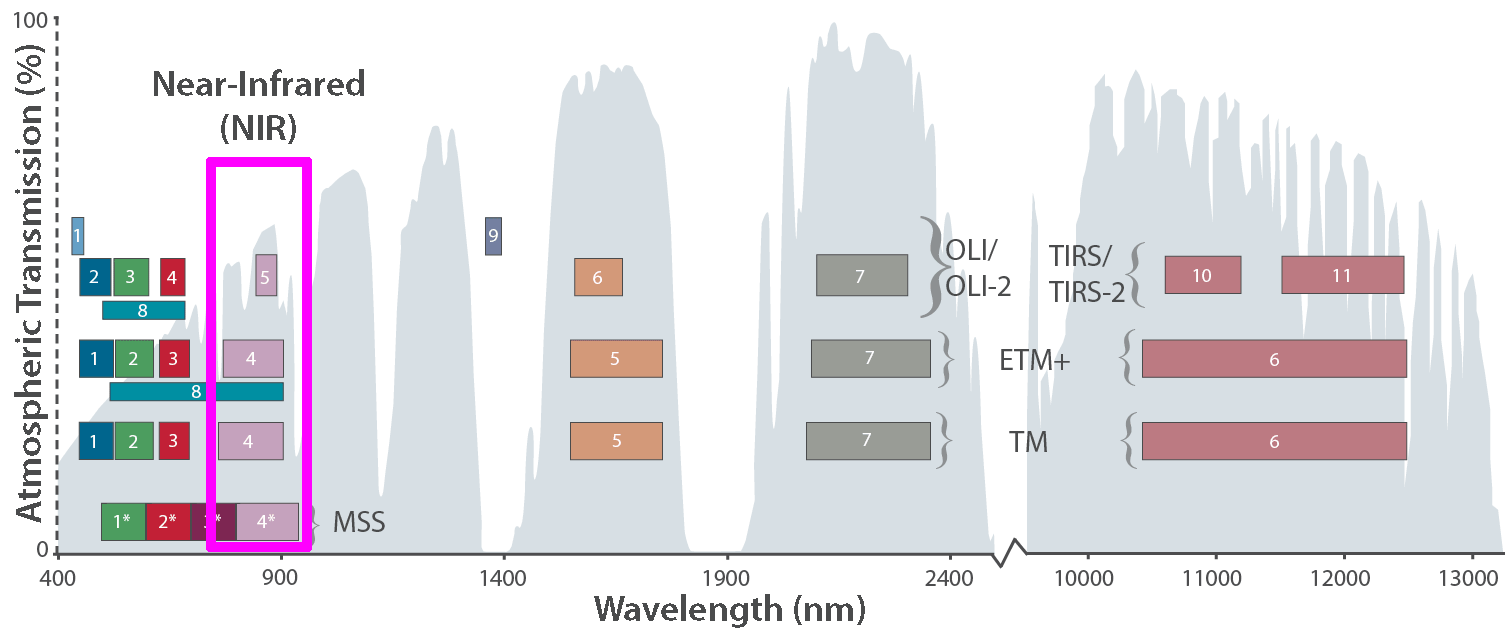
\includegraphics[width=9.0cm]{all_Landsat_bands_annotated.png}
    \caption{Landsat band availability overlaid a graph of atmospheric transmission percentages for various wavelengths. The Near-Infrared The NIR band (highlighted in pink) benefits from both long time series availability, as well as high atmospheric transmittance.}
\end{minipage}
\end{wrapfigure}

We evaluate several potential dataset sources that provide raw data from which we assimilate calving front positions. These include Terra/MODIS, TerraSAR-X, Landsat, and Sentinel. We compare the potential data sources' attributes in Figure 1. We select Landsat for its long time-series availability and reasonable spatial resolution.

We constrain our input to be based on subsets of a single band. This is due to the computational constraints of processing multiband inputs, and differences between available bands across Landsats 1-8. Another consideration is the diminishing returns of adding additional bands. Since pixel information is correlated across different bands, and since a single band image already shows any discernible calving fronts, additional band information was deemed unnecessary.

%Insert landsat band overlap table
%https://landsat.gsfc.nasa.gov/landsat-9/landsat-9-spectral-bands/
We pick the Near Infrared (NIR) (.77-1.1$\mu m$) wavelength band. This is based on evaluating  Landsat 1 - 8 band commonality, and choosing the band with the longest time series availability (See Figure 2). We then pick the band with the highest atmospheric transmittance, which allows us to "look past" light cloud cover. We initially hypothesized that using a common band is beneficial, as different spectral bands may exhibit features differently, and thus negatively impact detection accuracy. However, in practice (see 7.3 Discussion - Inter-model Comparison), the band selection is inconsequential as long as calving fronts are visible.

%%FIX THESE FIGURES - UPDATE TEMPORAL RESOLUTION & ADD TO SPATIAL COVERAGE MAPS

\begin{wrapfigure}{r}{12.1cm}
    \noindent
    \begin{minipage}{4.8cm}
        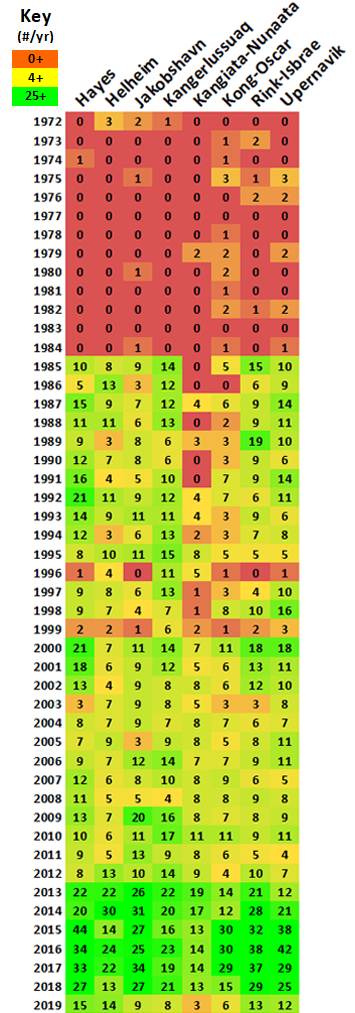
\includegraphics[width=4.8cm]{temporal.png}
        \caption{Number of images across the years for 6 selected glaciers. We evaluate glaciers across a longer time series than any existing studies.}
    \end{minipage}
    \hspace{0.15cm}
    \begin{minipage}{7.15cm}
        \centering
        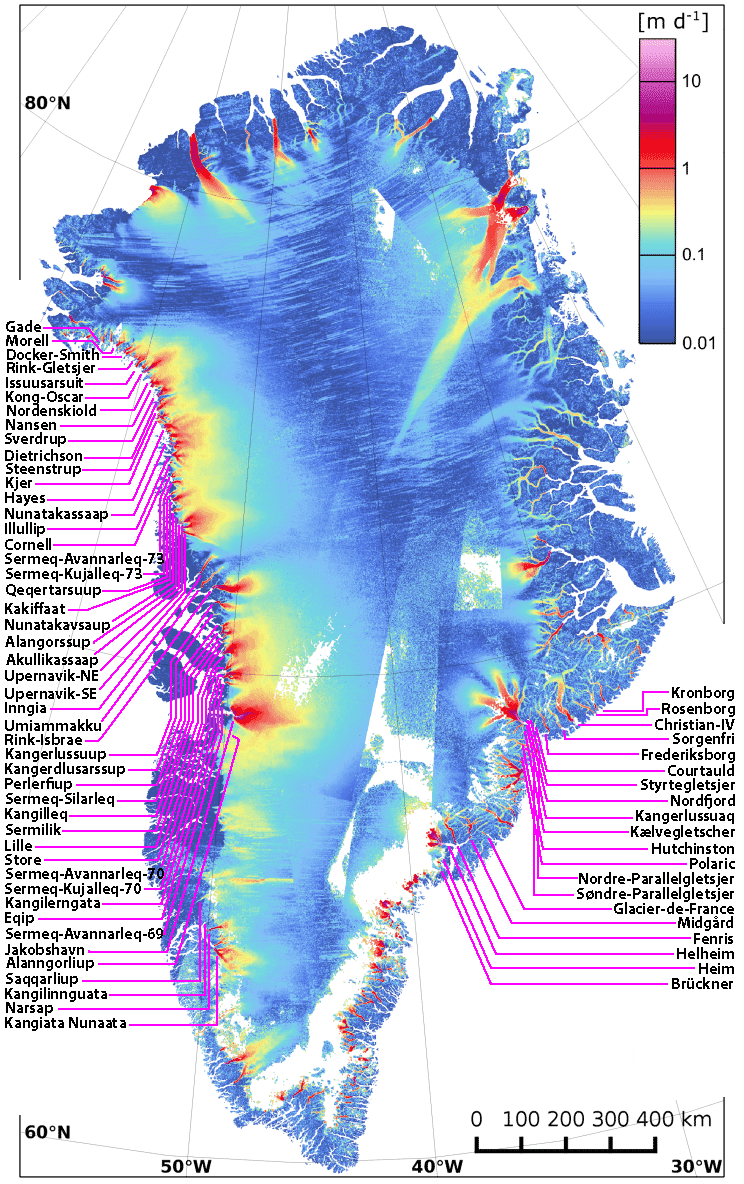
\includegraphics[width=7.15cm]{spatial_66.png}
        \caption{Spatial distribution of 66 glaciers along West Greenland. We study glaciers with reasonable velocities and wide spatial distribution.}
    \end{minipage}
\end{wrapfigure}

\subsubsection{Time Series Coverage}
Landsat availability per year, for all 6 basins. 
Gaps are due to clouds or lack of classifier confidence.
Color key shows rough number of observations per year.
See Figure 3.

\subsubsection{Spatial Coverage}
CALFIN data availability along West Greenland, for the highlighted basins, over velocity map \citep{nagler2015}.
Basins are primarily selected for study potential/high velocities.
Basins are secondarily selected for equal sampling of coastline.
See Figure 4.

\subsection{Data - Preprocessing}
Throughout our study, we developed a pipeline that automates much of the data preprocessing that is required for this task. This pipeline involves the following steps: Data source collection, GeoTIFF/domain subsetting, Low quality/clouded image pruning, Subset standardization, Detail Enhancement.
Once these steps are complete, we proceed with processing in the neural network processing step. See Figure 3 for a visual outline of these steps.


\begin{figure}[t]
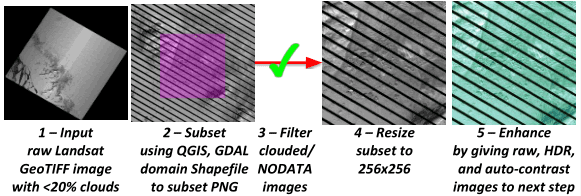
\includegraphics[width=14cm]{pipeline-preprocess.png}
\centering
\caption{A visual outline of preprocessing steps. Each is explained in more detail in the following subsections.}
\end{figure}

\subsubsection{Data - Preprocessing - Collection}
As a first step, we collect the input raster images that for which we want to evaluate. We begin by selecting all rasters centered around  one of 8 primary glacial basins along East/West Greenland. These basins include Kong Oscar, Hayes, Rink Isbrae, Upernavik, Jakobshavn, Kangiata Nunaata, Helheim, and Kangerlussuaq. These basins are selected both for their spatial distribution as well as their high flow velocities. These characteristics are important for ensuring wide spatial coverage and having dynamic calving fronts. For each domain, we filter for all Level 1 TP rasters. We add selected L1GS/L1GT products, which we manually georeference, to fill in Landsat 1-2 time series gaps (1972-1985). We further filter for rasters with less than 20\% cloud cover across the entire area. At this stage, we accumulate a total of 4776 Landsat rasters, from which we subset individual glacial domains. 

\subsubsection{Data - Preprocessing - Subsetting}
To begin subsetting, we define the domain of a glacial basin, which should fully encloses the calving front being extracted. We encode the domain as a rectangular Shapefile polygon. Next, we automatically subset the raster for every time step which we want to evaluate for the domain. We repeat this process for each basin to be studied. While this requires manual input, it only needs to be done once, as the domains will be reused across multiple subsetting operations. For rasters and domains in West Greendland, we reproject to WGS 84 / UTM zone 21N (EPSG:32621). For East Greenland, we use WGS 84 / UTM zone 24N (EPSG:32624).

\subsubsection{Data - Preprocessing - Pruning}
After subsetting, we automatically prune images that are ill-suited for further processing. First, we determine the amount of NODATA pixels present in the subset, and remove it from evaluation if it exceeds a predetermined threshold (>30\%). This allows us to process images with Landsat 7 scan-line errors and domains along raster boundaries, while still filtering out largely out-of-bounds subsets. This prevents them from being unnecessarily and inaccurately processed. Also, if an accompanying Quality Assurance band is present, the same filtering procedure is performed to eliminate images with high cloud cover, for the same reasons. We accumulate 20,029 GeoTIFF subsets, spread across 66 glacial domains.

\subsubsection{Data - Preprocessing - Standardization}
Now we resize the image to a standardized, square resolution. We convert the subsets from their native GeoTIFF formats to a standardized 256x256 PNG image. This step can introduce error into the delineation, which we address by defining domains as close to the square aspect ratio whenever possible.

\subsubsection{Data - Preprocessing - Detail Enhancement}
Lastly, we perform image transformations to enhance detail and provide the processing step with more information. We found through empirical testing that this step can specifically benefit raw images with heavy shadowing. This benefit emerges since these images contain details which are otherwise undetectable by the filters used in the processing step. We utilize two non-linear transformations, the Pseudo-HDR Toning and Shadows and Highlights enhancements. These enhancements are performed with default settings in Adobe Photoshop, but we aim to write an open-source equivalent in Python in the future. We concatenate the results of the two transformations with the raw image. This creates 3-channel RGB input images that contains information to be be utilized by the next step. 

At this point, the images are ready for processing into calving front masks.


\section{Methodology - Processing}
We perform the core processing step by passing images through the Calving Front Machine Neural Network (CALFIN-NN). As a convolutional neural network that inherits from the U-Net family of architectures, CALFIN-NN is capable of learning abstract image features, and outputting confidence masks of where it detects coastlines  and calving fronts. Importantly, it generalizes to new data automatically. This key capability is the foundation of most other automated methods in this field, including those by Zhang \citep{zhang2019}, Mohajerani \citep{mohajerani2019}, and Baumhoer \citep{baumhoer2019}.

Our network builds upon this work, and utilizes a modification of Google's DeepLabV3+ Xception \citep{chen2018} image segmentation network. With our customized architecture and training regimen, CALFIN-NN is capable of handling inputs with different scales/resolutions, heavy shadowing, ice mélange, light cloud cover, and Landsat 7 scan-line errors. Together, these novel innovations bring the state-of-the-art in image segmentation to the cryosphere community.

Our implementation of this processing step begins by splitting up the 256x256x3 pre-processed images into 9 overlapping 224x224x3 image patches. We exploit the overlapping windows to allow for both a smaller network size, as well as  to create a confidence estimate in our predictions over multiple processing passes per pixel.

After processing each input image, the  outputting a coastline/calving front mask is ready to be post-processed.

The following section goes into additional detail regarding aspects of our neural network model. Further details - including the iterative process of testing, evaluation methods, and our final training regimen - are described in Discussion. 

\subsection{Model Architecture \& Modifications}

\begin{figure}[t]
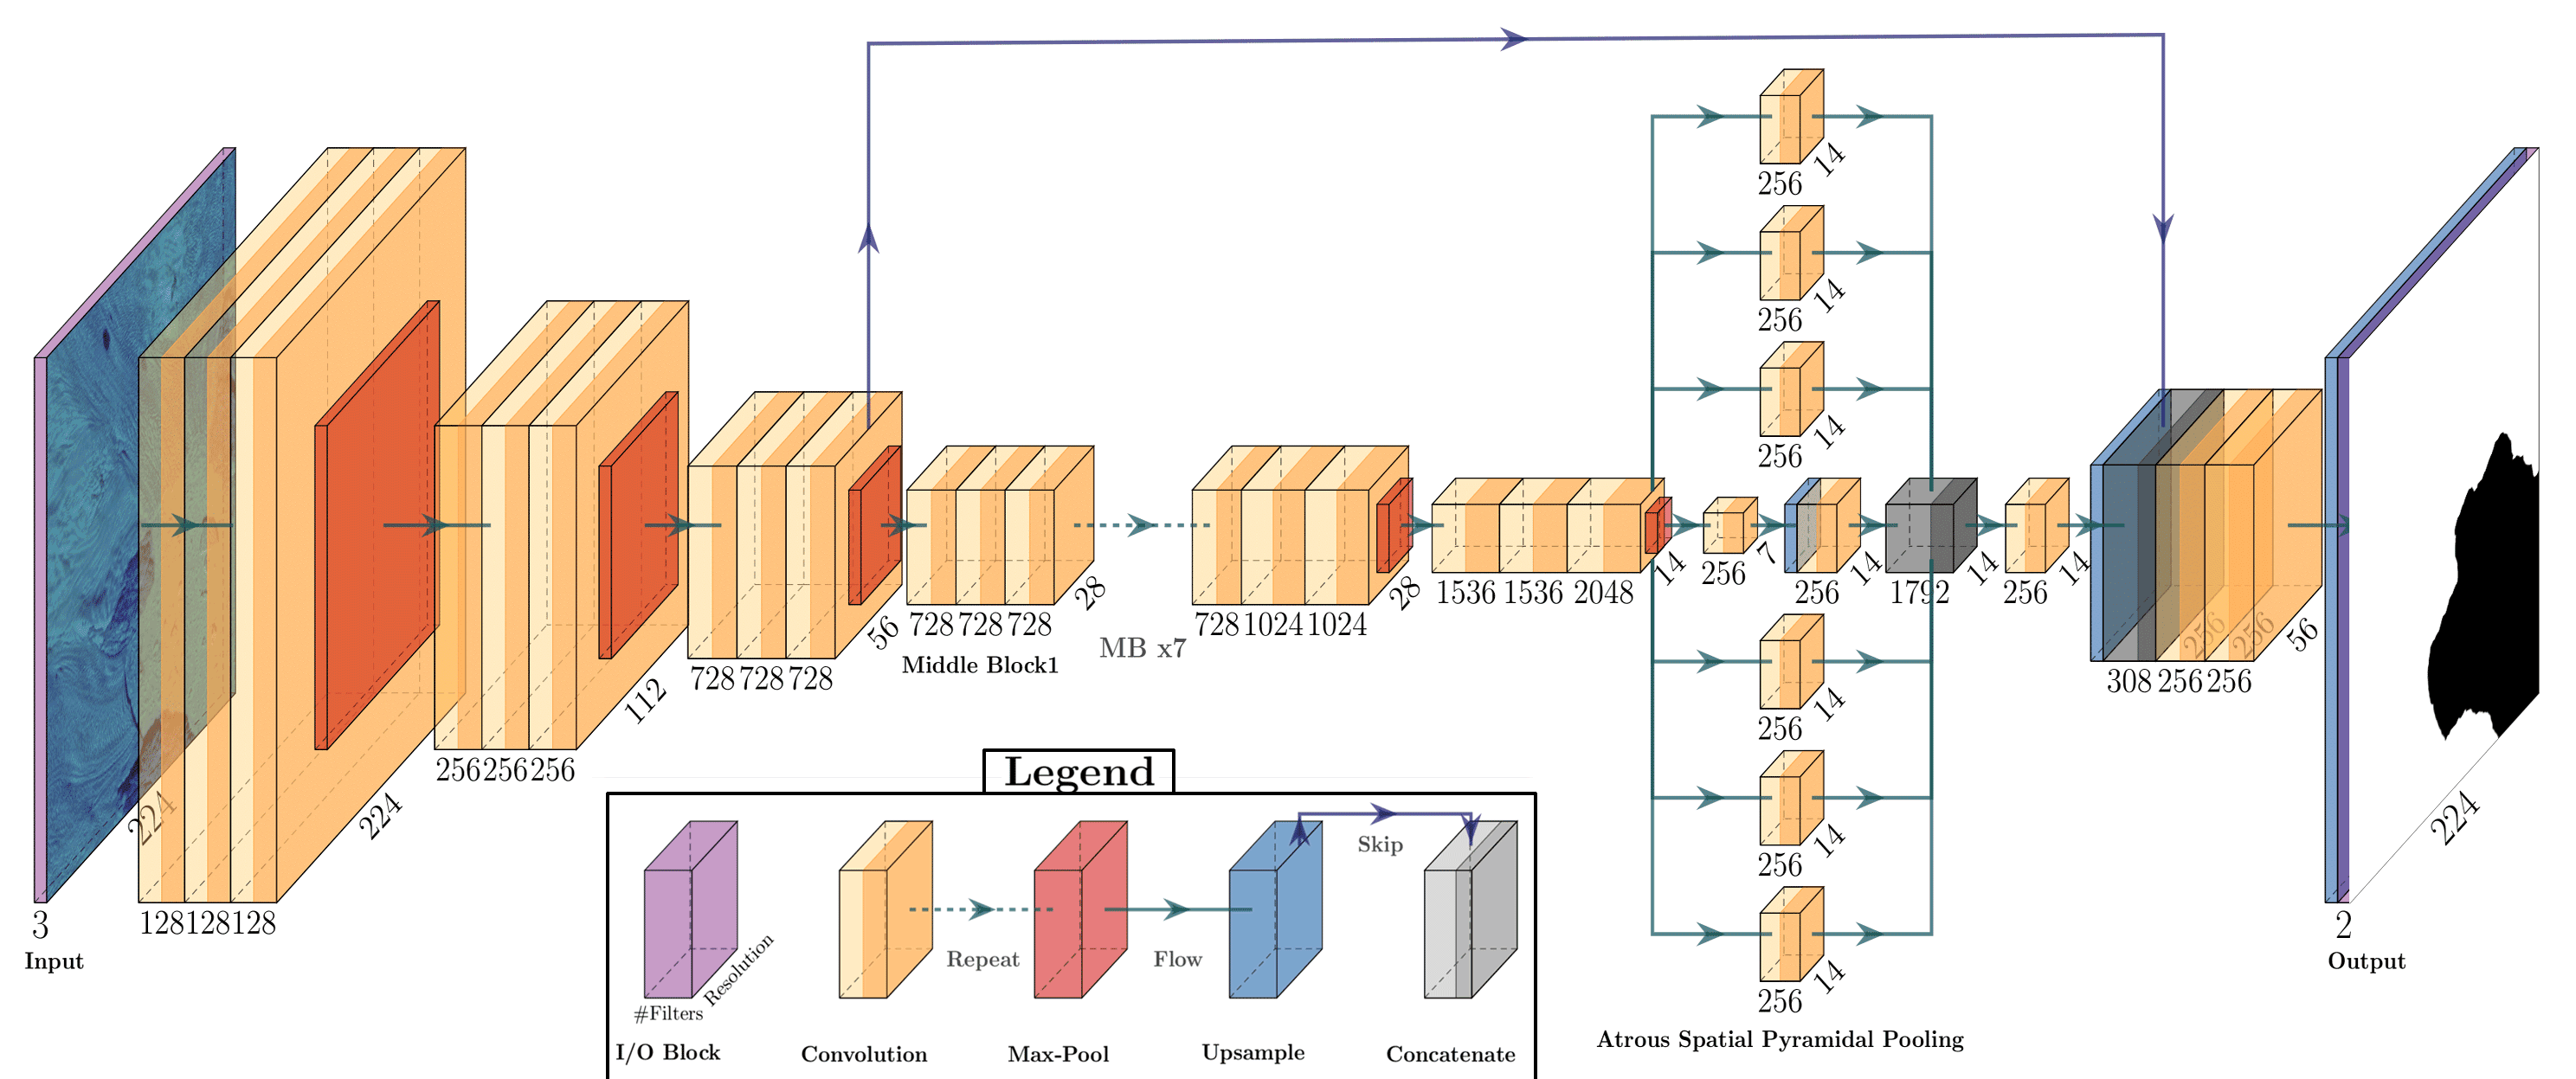
\includegraphics[width=18cm]{arch_final.png}
\centering
\caption{CALFIN-NN model architecture. The first half, the encoder, consists of multi-scale feature extraction blocks (Orange Xception modules, Atrous Spatial Pyramidal Pooling block). Note blocks in the middle flow section have been omitted for clarity (MB x7 represents 7 more sequential middle blocks). The second half, the decoder, up-scales the features and localizes the calving front at higher resolutions. CALFIN-NN belongs to the UNet family of architectures, and inherits directly from the DeepLabV3+ Xception network.}
\end{figure}

CALFIN-NN takes in 3-channel pre-processed images, as detailed in section 2.2.5.
CALFIN-NN outputs 2-channel images containing the coastline/calving front edge in the first (Red) channel, and the land ice/ocean mask in the second (Green) channel.
The model architecture consists of a modified DeepLabV3+ Xception image segmentation network, as shown in Figure 5. 
The first half of the network - the encoder - uses the Xception-65 network \citep{chollet2016} as our feature extractor. These features encode information in the image using higher-order image kernels. In other words, it assembles basic features (such as edges, corners) into more abstract features (such as glacier/land textures). DeepLabV3+ adds in a Atrous Spatial Pyramidal Pooling (ASPP) module that further enhances multi-scale feature detection, as each separate block in the ASPP module uses kernels dilated to a different scale. 
The second half of the network - the decoder - takes the output of the encoder and the ASPP module, up-samples the features and predicts the final output before performing one last up-sampling to the original input/output size. Note that no additional convolution kernels are used after the final up-sampling, and the usage of 4x up-sampling instead of 2x up-sampling. See the DeepLabV3+ paper by Chen et al. for insight into the reasoning for these design decisions \citep{chen2018}.

We make several modifications to the basic DeepLabV3+ Xception model architecture. Since DeepLabV3+ Xception is optimized for segmenting and classifying objects, it requires changes to accurately recognize thin/line features like calving fronts. To this end, we add additional ASPP blocks with different dilation scales (6, 12, 18 in the original, compared to 1, 2, 3, 4, 5 in CALFIN-NN). Furthermore, we modify the deepest pooling layer to only downsample by 2 instead of 14. These changes account for differences in input size when compared to the original model (224 vs 512) and enable better multi-scale feature localization. We switch the encoder module from the Xception 71 layer model to the Xception 65 layer model and remove the header module of DeepLabV3+, as both reduced the resolution of the image too much for accurate edge localization. We also modified tail of the network to output 2 channels for mask and edge simultaneously. These changes both reduce the weight size from ~40m parameters to ~29m parameters (~400MB on disk) as well as increase the overall accuracy of the network.

Ultimately, these modifications and the neural network architecture itself are the key innovations that allows for automatic processing of calving front images.

\section{Post-Processing}
At this stage, the 2-channel pixel mask output of CALFIN-NN must be post-processed in order to create a useful data product. However, this task is non-trivial, and is subject to several unique constraints. We describe the various problems we encounter, and offer our unique solutions for each.
\begin{itemize}
\item The pixel mask output by CALFIN-NN is often imperfect. We develop a unique algorithm to infer the correct coastline boundary.
\item The calving front must still be isolated from the coastline that is output by CALFIN-NN. We utilize fjord boundary masks and image analysis techniques to accomplish this.
\item The isolated calving fronts must then be isolated and refined, as the fixed input/output resolution of CALFIN-NN results in error associated with subset rescaling. We address this by performing a pseudo box-regression, and re-processing zoomed-in subsets that are centered on each isolated calving front.
\item Each refined calving front must still be transformed into a georeferenced Shapefile for further use. This is comparatively easy to solve using GDAL and the original GeoTIFF subsets, but still must be performed.
\end{itemize}
The following subsections cover our solutions to each of the problems above. See Figure 7 for a visual outline of these steps.

\begin{figure}[t]
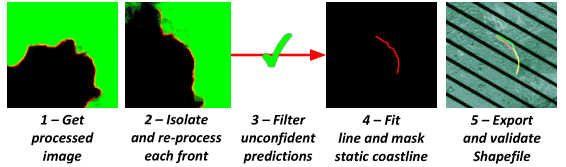
\includegraphics[width=14cm]{pipeline-postprocess.png}
\centering
\caption{A visual outline of postprocessing steps. Each is explained in more detail in the following subsections.}
\end{figure}

\subsection{Post-Processing - Pixel Mask to Coastal Polyline}
The first problem is that the raw pixel mask is often imperfect. Currently, CALFIN-NN cannot always completely determine the calving front in an arbitrary image. As a consequence, traditional vectorization methods using OpenCV or GDAL will not work with the imperfect, non-closed contours seen in  CALFIN-NN's output. However, the nature of its inaccuracies are predictable. Thus we exploit the characteristics of CALFIN-NN's output to compensate for its specific inaccuracies. $show examples here!$

To address this first constraint, we develop an algorithm that finds the polyline representing the coastline in the pixel mask. This is implemented by converting each pixel in the mask to nodes in a graph, and finding the single longest path in the graph's minimum spanning tree. This path consistently corresponds to the the coastline edge. Note that this algorithm is not guaranteed to find the correct calving front, as is still limited by the output of processed by CALFIN-NN.

A detailed explanation of the algorithm follows below.

%Include figure of pipeline here

\begin{enumerate}
    \item First, calculate the euclidean distances between each node and every other node, creating distance matrix D.
    \item Then for each point, find the k-nearest neighbors using distance matrix D. K is generally chosen to be the maximum of some minimum number of nodes (we choose 4) and some percentage of the total number of nodes (we choose 20\%). The choice of K for following outlier detection step.  This step ensures continuous lines, removes some outlier noise, while still allowing for large gaps in the pixel mask graph to be crossed.
    \item To further address outliers and spurious detections, we remove any nodes that mean distance to its neighbors is itself an outlier. To compute the outliers of mean neighbor distance, we use the robust Modified Z-score method with Median Absolute Deviation \citep{garcia2012}. We eliminate any node whose mean neighbor distance exceeds a z-score of 10. We determine this threshold through empirical testing. 
    \item Next, we use the k-nearest neighbors graph to construct a undirected weighted minimum spanning tree (MST).
    \item Lastly, we find the longest path in the MST. This can be done by performing 2 depth-first searches (DFS), with each DFS finding one endpoint along the longest overall path. This longest overall in the MST consistently corresponds with the calving front detected by CALFIN-NN.
\end{enumerate}

\subsection{Post-Processing - Coastline to Calving Front}
The second problem is to isolate the calving front from the coastline polyline output by the previous post-processing step. This problem occurs because CALFIN-NN is trained to detect ice/ocean boundaries, but not yet how to isolate the fronts themselves. Therefore, work must be done to remove edges detected along the fjord boundaries.

We address this second constraint by creating 66 fjord boundary masks, one for each domain. We then use these masks to extract the front from the full coastline edge mask that is output by the neural network. Still, due to coastline variations, the static fjord boundary mask does not always isolate the calving front. Thus we develop another algorithm to contract the boundary mask until only the calving front remains. We exploit the fact that the detected coastline is parallel to the fjord boundaries, while the calving front is usually perpendicular to both. Following this step, each calving front terminates near the fjord boundaries, and is ready for further post-processing. In our future work, this step can be integrated directly into the neural network. This can be done by adding a third output channel that discards coastline/fjord boundaries and only contains the isolated calving fronts.


%A detailed explanation of the algorithm follows below.

%Include figure of pipeline here

%\begin{enumerate}
%    \item TOFIX
%\end{enumerate}
%show erosion steps here, with highlight around optimal

\subsection{Post-Processing - Calving Front Reprocessing}
The third problem arises from the fact that our image subsets encompass the entire range of potential calving fronts over the period 1972-2019. This results in lower accuracy when extracting the calving front, due to the lower spatial resolution of the input imagery.

We address this third constraint by exploiting CALFIN-NN's multi-scale capabilities, and reprocessing a subset of the image subset. We perform this operation doing a second processing pass, where the first one detects the fronts, and the second one "zooms in" on each detected front. This implementation mimics a bounding box regression and localization routine commonly found in other neural networks. Furthermore, each individual front may or may not be confidently detected. We exploit the nature of CALFIN-NN's output as a confidence measure, so that generated fronts can be filtered out based on confidence thresholds, and overall accuracy can be increased. In the future, this step can be integrating directly into the neural network. 

\subsection{Post-Processing - Calving Front to Shapefile}
The last problem is to correctly transform the vectorized polyline to a geo-referenced Shapefile. While this problem is more easily solvable, it must still be performed in order to generate the desired data product. Additionally, there may be multiple fronts depending the specific domain and time frame. %Show example

We address this last constraint by using GDAL and the GeoTIFF subsets from the preprocessing step to re-scale the polyline, georeference it, and export a Shapefile data product.


\section{Analysis Methodology}
We have two primary methods of evaluating the predicted output of any calving front against the ground truth labeling.
The first method is the standard Intersection over Union, or Jaccard index. This is the same metric used by Baumhoer et al. \citep{baumhoer2019}. This metric evaluates the degree of overlap between the predicted and ground truth pixel masks of the calving front. It is calculated by dividing the number of pixels in the intersection of two masks over the number of pixels in the union of the two masks. When calculating the IoU between 3 pixel wide edges, this measure is very conservative: 1 pixel of difference results in a score of 0.5000, and scores in that range and above are indicative of human level accuracy. When calculating the IoU between large land/ice-ocean-mélange masks, this measure is less conservative, and scores in the range of 0.9000 and above are indicative of human level accuracy.

The second method is the more domain specific Mean Distance from the Front. This is the same metric utilized by Mohajerani et al.\citep{mohajerani2019} Zhang et al. \citep{zhang2019}. This metric evaluates the average distance between closest points between predicted and ground truth fronts. Conceptually, this method resembles numerical integration of the area between two curves, divided by the average length of the curves. This metric is implemented TODO


\section{Results}
We generate results that are two-fold in nature. First, we release the an implementation and error analysis of CALFIN-NN to the scientific community for use, study, and further development. Second, we release the calving front data we generate throughout the study, which consists of approximately 1500 manually delineated calving fronts across 66 Greenlandic glacial domains.

%Data outputs:
%	CALFIN Neural Network
%		Weights, Architecture
%	Calving Fronts
%        Level 0: Raw subsets, neural network %masks
%        Level 1: Shapefiles

\subsection{CALFIN Neural Network Error Analysis}
For our error analysis, we manually delineate 152 validation images that are not used for training the network, and compare the output of the predictions versus our manually delineated ground truth images. Our validation image is a representative sub-sample of our overall training data, and similarly spans from 1972-2019 across over 60 glacial domains. We utilize two primary means of evaluating accuracy, which are also utilized by existing work in the field \citep{mohajerani2019} \citep{zhang2019} \citep{baumhoer2019} and can be used for inter-model comparison (see section 6.3, Discussion - Inter-model Comparison). These are the mean distance between the predicted and ground truth fronts, and the Jaccard index.

We achieve 102.27 meters mean distance between the predicted and the ground truth front over our validation set of 152 manually delineated images. 

We achieve a mean Jaccard index (Intersection over Union) of 0.5281 between our 3-pixel wide predicted and ground truth fronts.

We achieve a mean Jaccard index (Intersection over Union) of 0.9472 between our  predicted and ground truth land/ice-ocean/mélange masks.

We were able to detect fronts in 82.24\% of the validation set (125 out of 152)

We were able to detect fronts in 90.58\% of the validation set when accounting for test images where there was no front in the ground truth (125 out of 138).

The methodology behind these accuracy evaluation metrics is detailed in the subsequent subsection.

\subsection{Results - Manually Delineated Fronts, Training Data}

%Show layered fronts for 1 or 8 domains
%Show accuracy metrics, list numbers of subsets

%Retrieve graphs from pyplot, showing mean deviation from front histograms
Approx 2k high res, hand-made/verified data (<30m accuracy from hand drawn line, but should be cross validated with other's data - see inter-comparison section). Derived from training data. 66 domains, ~4-50 data points for each domain
Approx 20k unverified test data ~40-500 data points for each domain
Shapefile

\section{Discussion}
We describe information, materials, and methods that are auxiliary to the data and methodology described in this study. This includes the following topics:
\begin{itemize}
    \item We document how our neural network was trained, to encourage transparency and reproduciblility.
    \item We talk about the existing work in this field, specifically surrounding deep learning applied to calving front/coastline extraction.
    \item We perform a model inter-comparison with Mohajerani et al., to study the robustness of both models and their evaluation metrics.
\end{itemize}

\subsection{Discussion - Neural Network Development and Training}
\subsubsection{Training Data}
In order to train our network, we create training data, which consists of preprocessed inputs and ground truth images. This training data consists of 1744 images pairs, with 1555 pairs for training and 189 pairs for validation. 
\subsubsection{Network Architecture Search}
We began our search using the same basic UNet architecture as found in Zhang et al.\citep{zhang2019}, Mohajerani et al.\citep{mohajerani2019}, and Baumhoer et al.\citep{baumhoer2019}. During our initial development, we varied the UNet's depth, number of filter layers, and input size. However, as we added more domains and poorer quality images, it became apparent that the network architecture was limited. 
At this point, we decided to evaluate other state-of-the-art image segmentation networks. We found Google's DeepLabV3+ Xception network to be the highest performing architecture on common benchmark segmentation datasets such as PASCAL-VOC. The DeepLabV3+ Xception architecture shows improvements in multi-scale feature extraction at a reasonable computational cost as compared to UNet derived architectures. Additionally, its larger size gives it the capacity to learn much more abstract features - this improvement is essential for addressing issues like shadows, ice mélange/buttressing, and Landsat 7 scan-line errors.

To improve accuracy further, we modified the DeepLabV3+ Xception network. 

\subsubsection{Training Regimen}
We trained the network over 80 epochs, with 4000 batches per epoch, and 8 images per batch. We utilized a K40 Nvidia Tesla GPU, with each epoch taking 7540 about 126 minutes to complete, or about 1 week to complete all 80 epochs. We utilize the Adam optimizer, which automatically computes optimal learning rates per parameter. We do use a modified Adam optimizer that accumulates the gradient over 2 batches so that our effective batch size is 16. Additionally, it clips the learning rate at 1e-4, to prevent exploding gradients during training/backpropagation.
We utilize Exponential Linear Units (ELU) over ReLU as our activation function, to prevent vanishing gradients. Our loss function is a weighted combination of binary cross entropy (BCE) and two Jaccard/Intersection-over-Union (IoU) calculations. 
%Insert equation here
This loss function heavily penalizes incorrect predictions (a property of BCE/IoU), heavily favors correct predictions (a property of IoU), and is differentiable (a property of the natural log). Additionally, the weighting heavily favors correct coastline/edge mask predictions, which is critical for increasing calving front prediction accuracy.
\subsubsection{Data Augmentation/Test-time Augmentation}

\subsection{Discussion - Existing Work}
Our work was performed alongside - and builds on - existing work done in the field.

Mohajerani et al.\citep{mohajerani2019} provides a similar case study using the same type of deep neural network architecture to detect calving fronts. His study is performed on the Greenlandic glacial basins Jakobshavn, Helheim, Sverdrup, and Kangerlussuaq. Mohajerani's methodology displays promising steps towards generalizability and has been preeminent in the field.

Zhang et al.\citep{zhang2019} performs an analysis similar to Mohajerani, albeit in a more specific case study using SAR data of Jakobshavn. The applicability of neural networks as a general methodology for calving front analysis is supported by its successful usage here. 

Baumhoer et al.\citep{baumhoer2019} evaluates modified UNet architectures, as applied to SAR data of Antarctica. Her studies incorporate large spatial context in order to capture whole-coastline delineations. The prospect of larger networks on the order of 768x768 pixels offers the promise of higher resolution/accuracy outputs.

Our methodology shares the same basic approach with the above. We utilize an updated neural network architecture - DeeplabV3+ Xception - that improves upon the base UNet design. Furthermore, we use additional post-processing steps to make the detection more accurate.

\subsection{Discussion - Inter-model Comparison}
We perform an inter-comparison between the performance of CALFIN with respect to the existing studies. In particular, we conduct a comprehensive inter-model comparison between CALFIN and the model developed by Mohajerani et al. Together, these comparisons allow for a robust evaluation of different models and error quantification metrics for automatic calving front detection. To perform this task, we process the validation data used by each other's models, and compare the results.
%TODO
%have Yara/Mike insert results of preprocessed Helheim on Yara's network here?

\begin{figure}[t]
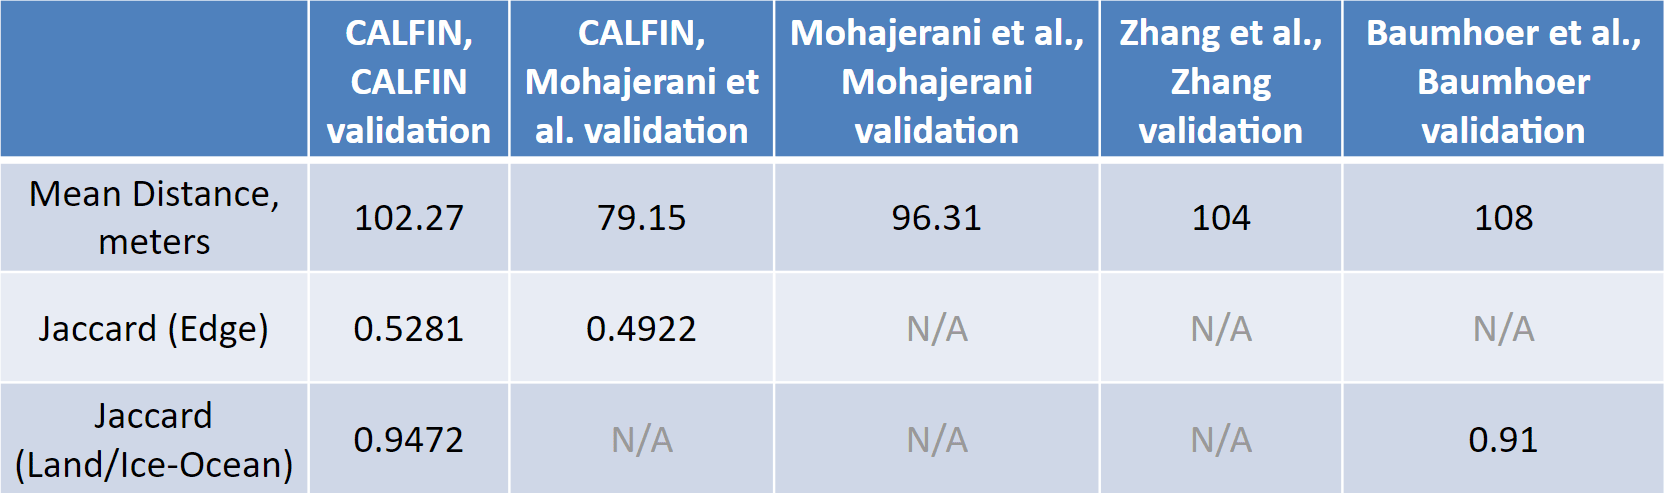
\includegraphics[width=16.0cm]{intercomp-table.png}
\caption{Distances between predicted points and the true front. Calculated over the 10 images from Mohajerani et al. Compare mean deviations from our method (102.52m) and Mohajerani et al. (96.31m). While our method is not as performant on this subset of images, the ability of our network to other domains and conditions is an acceptable tradeoff.}
\centering
\end{figure}

\begin{figure}[t]
\includegraphics[width=18cm]{helheim_plots_intercomp.png}
\caption{The graphs above provide verification information for a single test image from the set of 10 used in Mohajerani et al. \textbf{b)} is an RGB image containing the raw image (R), a High Dynamic Range toned image (G), and a Shadows/Highlights enhanced image (B). This prerocessed image is then fed into CALFIN-NN. \textbf{c)} is an RGB image, containing the coastline/edge mask (R) and the land/ice mask (G). \textbf{e)} compares the fronts from our method (R), the ground truth (G), and Mohajerani et al. (B). The Jaccard index calculates the overlap between our method and the ground truth as a percentage from 0 to 1. \textbf{f)} is a histogram that quantifies the error between our method and the ground truth. The error is quantified in terms of distance between each pixel in one line and the closest point in the other line.}
\centering
\end{figure}

\begin{figure}[t]
\includegraphics[width=16.0cm]{helheim_histo_intercomp.png}
\caption{Distances between predicted points and the true front. Calculated over the 10 images from Mohajerani et al. Compare mean deviations from our method (102.52m) and Mohajerani et al. (96.31m). While our method is not as performant on this subset of images, the ability of our network to other domains and conditions is an acceptable tradeoff.}
\centering
\end{figure}

Across the all 10 test images in Mohajerani et al., we attain a 102.52 meter (2.10 pixel) mean distance between the predicted and the ground truth fronts. This metric is calculated by finding the closest points from every other point between the predicted and the ground truth front pixel masks. We see that this approaches the level of accuracy achieved in the original study, which was 96.31 meters (1.97 pixels). While our method does not exceed this level of accuracy, it was still able to approach it with no further training done. We conjecture that the relatively higher resolution and the lack of wider context in the input image results in this performance gap.
%To validate this conjecture, we reevaluate our Helheim validation images at higher resolution subsets, but with the added context of the nearby terrain and surroundings. %TODO?



Furthermore, note that \citep{mohajerani2019} obtained the mean error estimate by breaking each delineated front to 1000 smaller segments within x`a small buffer from the fjord walls and calculating the mean deviation between the segments of the true and delineated fronts. Here we calculate the errors by getting the mean distance between each pixel of the delineated front and the closest pixel of the true front. This does not require the fronts to have the same number of pixels, as several pixels can be mapped onto one pixel. It is important to emphasize that the error results can be very sensitive to the error evaluation methodology. By comparing pixels directly, we avoid comparing line segments far from each other due to different lengths of the delineated and true fronts. In that sense, the line-segment methodology of \citep{mohajerani2019} provides a more conservative estimate as it relies on line segments being close to each other.

\textcolor{red}{talk about other differences: landsat stripes not included in training of M19 (Mohajerani et al 2019), M19 used different spectrum band for training, fewer training instances in M19, maybe talk about post-processing difference (least-cost path through front-segmented output, etc.}

Overall, this inter-comparison supports our hypothesis that our methodology is generalizing well and is sufficiently accurate.

\conclusions[]Conclusion \& Future Work]
The calving front data products are being released on rolling basis at www.ics.uci.edu/~dlcheng. %datadryad or NSIDC?
The neural network model is being released on https://github.com/daniel-cheng/CALFIN.

Overall, we accomplished our goal of implementing a method for the automatic calving fronts delineation. Our method utilizes the cutting-edge in deep learning architectures. Our method achieves robustness to minor cloud cover, Landsat 7 scan line errors, and illumination changes. We address issues with generalization through use of additional training data and an improved neural network architecture. We are competitive among existing work being done in this field.  

Future work includes extending CALFIN-NN to integrate 

Our data augmentation, network architecture, and post-processing methods all contribute to the success of our methodology. Ultimately, this work showcases the state-of-the-art in field of deep neural networks as applied to automated calving front detection, and provides a new database of calving fronts for the scientific community.

\subsection{Supplement}


\codedataavailability{
    The code used to automate the CALFIN pipeline is freely available here: https://github.com/daniel-cheng/CALFIN
    
   The data generated by CALFIN, including Level 0 and 1 data products, are freely available here: (datadryad link)
}


\authorcontribution{
    DC developed the code/model, carried out the data processing, and wrote majority of the manuscript.
    YM performed the model inter-comparison and assisted with the writing of the manuscript.
    EL provided direction for the overall study.
    IV assisted in organizing collaborators and model inter-comparison.
    MW performed the data preprocessing for the model inter-comparison.
    WH provided direction on the processing methodology, post-processing algorithms, and error analysis.
    EL, IV, and WH reviewed the manuscript and evaluated the results.
}

\competinginterests{
    The authors declare no competing interests.
}

\begin{acknowledgements}
    This work was conducted as a collaboration between NASA’s Jet Propulsion Laboratory and the University of California, Irvine. 
\end{acknowledgements}

\bibliographystyle{copernicus}
\bibliography{references.bib}  %%% Use the external .bib file (using bibtex).

\end{document}